\documentclass[11pt,a4paper]{article}
\usepackage[margin=2.5cm]{geometry}
\usepackage{graphicx}
\usepackage{booktabs}
\usepackage{amsmath,amssymb}
\usepackage[table]{xcolor}
\usepackage{enumitem}
\usepackage{hyperref}
\usepackage{fancyhdr}
\usepackage{titlesec}
\usepackage{float}
\usepackage{listings}

\definecolor{accent}{HTML}{2d3436}
\definecolor{codebg}{HTML}{f5f5f5}
\pagestyle{fancy}\fancyhf{}
\rhead{\small Girish Narayanan}
\lhead{\small LCAS --- Weekly Report}
\rfoot{\small\thepage}
\renewcommand{\headrulewidth}{0.4pt}
\titleformat{\section}{\large\bfseries\color{accent}}{}{0em}{}[\vspace{-0.3em}\rule{\textwidth}{0.4pt}]
\graphicspath{{assets/}}

\lstset{
  backgroundcolor=\color{codebg},
  basicstyle=\ttfamily\small,
  frame=single,
  framesep=4pt,
  xleftmargin=6pt,
  xrightmargin=6pt,
  breaklines=true,
  columns=fullflexible,
}

\begin{document}

\begin{center}
  {\LARGE\bfseries First Blind Attitude Inversion\\[0.2em] from Specular Glint Constraints}\\[0.5em]
  {\large Weekly Report --- 27 March 2026}\\[0.3em]
  Girish Narayanan
\end{center}
\vspace{0.5em}

% ============================================================
\section{Summary}

\textbf{Working end-to-end blind inversion pipeline.} From a single observed
light curve, recovers $\omega$ direction to ${\sim}2^\circ$ and magnitude to
$< 0.2\%$ in \textbf{5--7 minutes}. Tested on 6 trajectories: 4/6 succeed.

\begin{center}
\begin{tabular}{@{}lr@{}}
\toprule
Best result (seed 93) & $\omega$ dir $= 1.25^\circ$, $|\omega|$ err $= 0.01\%$ \\
Known limitation & $180^\circ$ attitude ambiguity (satellite N/S symmetry) \\
Failure mode & $< 10$ constraint epochs $\Rightarrow$ insufficient observability \\
\bottomrule
\end{tabular}
\end{center}

% ============================================================
\section{Pipeline}

Steps 1--4 are purely geometric (no BRDF/shadows). Step 5 invokes the full
ray-traced forward model.

\begin{lstlisting}
STEP 1: Peak detection
  peaks       = find_peaks(observed_lc, prominence > 0.3)
  |w|_est     = 0.040 * n_peaks + 0.042 deg/s       (rho=0.92, 13% err)
  specular    = peaks where mag < 6     (guaranteed +/-X alignment with PAB)
  bright      = peaks where 6 < mag < 9 (some normal aligned with PAB)
  anchor      = brightest specular glint -> 1-DOF circle in phi

STEP 2: Omega grid search                            [~100s, 16 cores]
  for each of 2000 dirs x 20 mags (|w|_est +/- 20%):
    propagate identity quat from anchor -> delta_q at constraints
    sweep 36 phi values x {+X, -X} anchors (vectorised)
    score: C = w_s * sum(1 - align_pmX)^2    at specular epochs
             + w_b * sum(1 - align_any)^2    at bright epochs
    keep best (phi, cost) per direction

STEP 3: Nelder-Mead refinement                       [~14s, 16 cores]
  refine top 20 grid results (3D omega, 360 fine phi bins)
  extract top 5 omegas x {+X, -X} best phi = 10 candidates
  back-propagate each to t=0

STEP 4: Geometric refinement + cluster detection      [~63s, 8 cores]
  L-BFGS-B on all 10 candidates (specular + bright alignment, no BRDF)
  sort by geo cost -> find first 10x gap -> low-cost cluster

STEP 5: Hi-fi LC scoring                             [~150s, 8 cores]
  full ray-traced LC for cluster members
  rank by MSE residual -> winner
\end{lstlisting}

\vspace{0.3em}
\begin{center}
\begin{tabular}{@{}llr@{}}
\toprule
\textbf{Step} & \textbf{What} & \textbf{Time} \\
\midrule
1 & Peak detection + constraints & $< 1$\,s \\
2 & Grid search (2000 $\times$ 20, 36 $\phi$, vectorised) & 98\,s \\
3 & NM refinement (top 20, 360 $\phi$) & 14\,s \\
4 & Geometric refinement + cluster detection & 63\,s \\
5 & Hi-fi LC (cluster members) & 153\,s \\
\midrule
  & \textbf{Total} & \textbf{5.5\,min} \\
\bottomrule
\end{tabular}
\end{center}

\noindent\textbf{Key ideas:}
\begin{itemize}[nosep]
  \item \textbf{Delta-$q$ factorisation:} propagation is $q$-independent for
    torque-free dynamics. One propagation per $\omega$ serves all 360 $\phi$
    candidates.
  \item \textbf{Specular $\Rightarrow$ $\pm X$:} every mag $< 6$ peak is a
    $\pm X$ face alignment (100\% across 6000+ peaks). This constrains
    attitude to a 1-DOF circle per glint.
  \item \textbf{Cluster detection:} geometric cost separates viable candidates
    from junk (typically $10$--$75\times$ gap). Only the cluster gets the
    expensive hi-fi evaluation.
\end{itemize}

% ============================================================
\section{Candidate Disambiguation}

\begin{figure}[H]
\centering
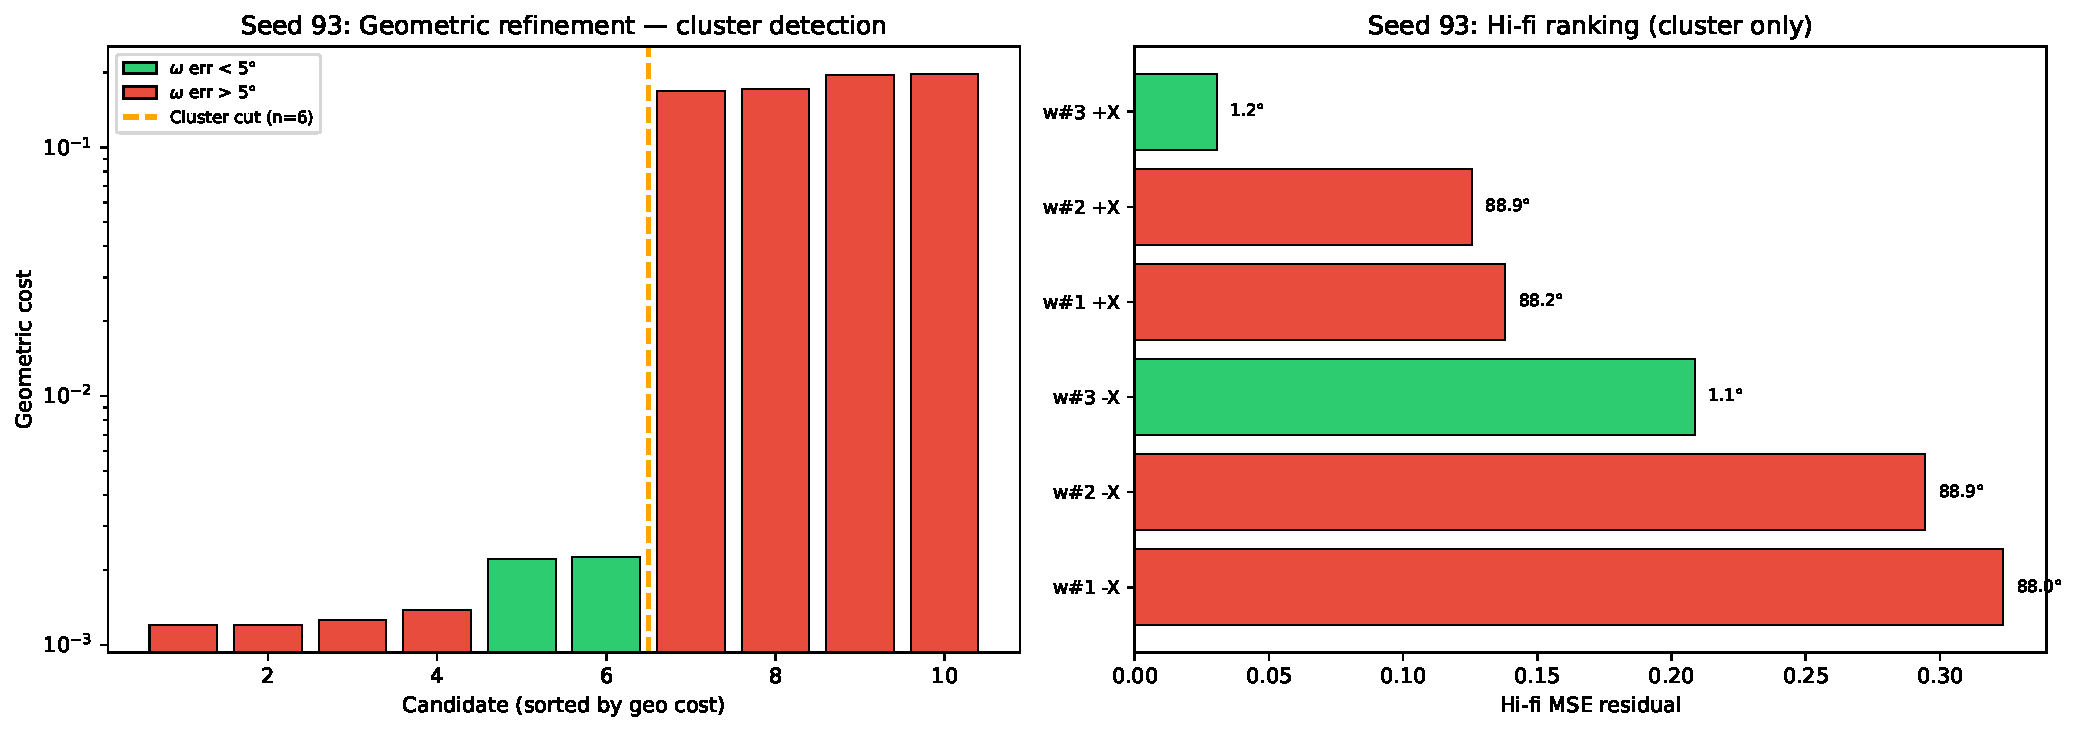
\includegraphics[width=\textwidth]{hifi_cluster_seed93.pdf}
\caption{Seed~93. Left: geometric cost (log scale) --- 6 candidates below
the 75$\times$ gap. Right: hi-fi residual ranks correct $\omega$ at \#1
with $4\times$ margin.}
\label{fig:cluster}
\end{figure}

% ============================================================
\section{Geometric Degeneracy}
\label{sec:degeneracy}

IS-901 has \textbf{mirror symmetry about the body $XY$ plane}: the north
and south solar panels are identical, and the bus is symmetric above and below.

\begin{itemize}[nosep]
  \item For any $\phi$, the attitude at $\phi + 180^\circ$ swaps N/S panels
    $\Rightarrow$ nearly identical satellite geometry and light curve
  \item $\omega$ recovery is unaffected (both $\phi$ values yield the same
    $\omega$)
  \item $q_0$ differs by ${\sim}180^\circ$ between the two
  \item This is a \textbf{true geometric degeneracy} of the satellite shape
    --- not a pipeline limitation
  \item \textbf{Fix:} sample $\phi \in [0^\circ, 180^\circ)$ instead of
    $[0^\circ, 360^\circ)$. This eliminates the duplicate and halves the
    phi search space with no loss of information.
\end{itemize}

\noindent Note: the $\pm X$ anchor ambiguity (front vs back of the bus) is a
\emph{separate} question. The front and back of IS-901 are \emph{not} symmetric
(different dish/antenna geometry), so $\pm X$ disambiguation is feasible via
hi-fi residual comparison. The pipeline already handles both $\pm X$ anchors
internally.

\begin{figure}[H]
\centering
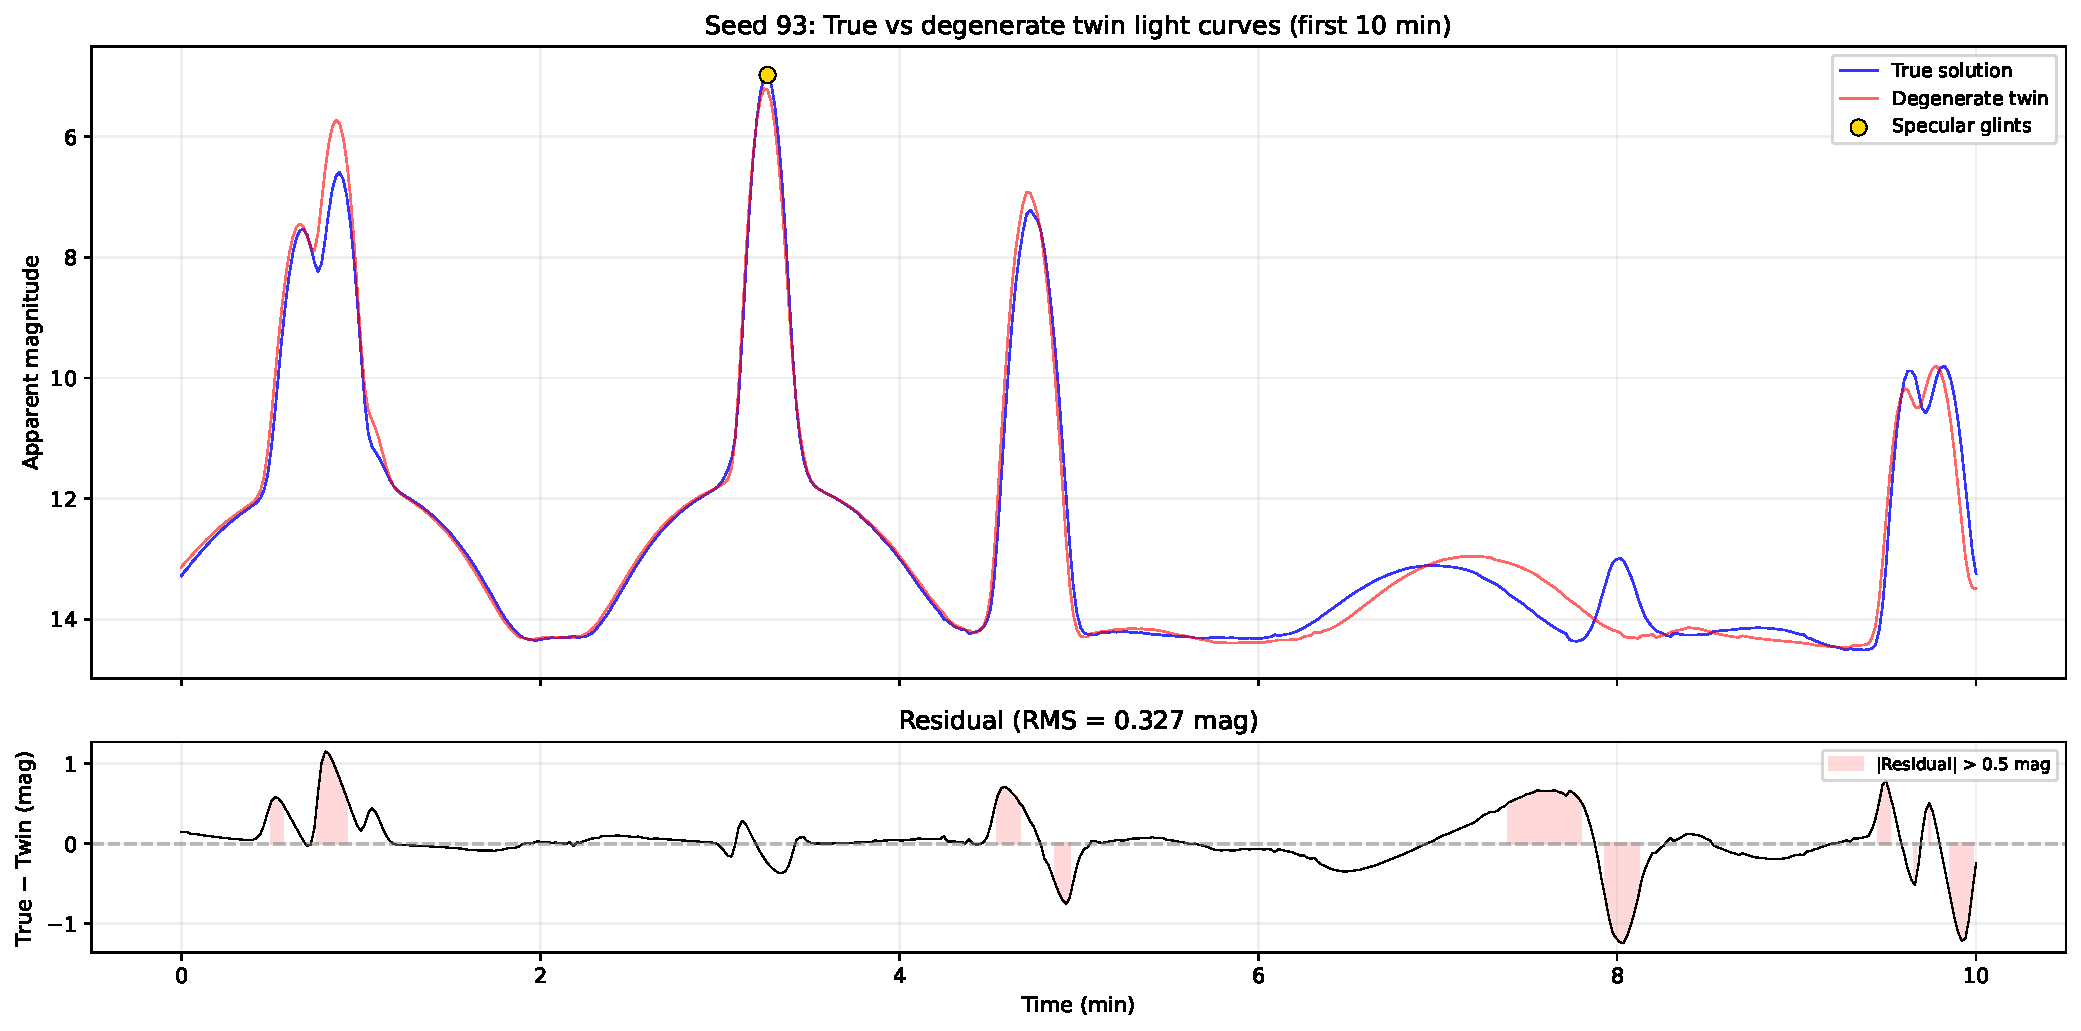
\includegraphics[width=\textwidth]{lc_twin_comparison.pdf}
\caption{True (blue) vs degenerate twin (red, $179^\circ$ offset, same
$\omega$). Specular glints (gold) match by construction; differences appear
in shadow-driven dim epochs.}
\label{fig:twin}
\end{figure}

% ============================================================
\section{Multi-Seed Results}

6 trajectories, $|\omega| \in [0.85, 1.45]$\,deg/s, $\geq 3$ specular glints each.

\begin{table}[H]
\centering
\small
\caption{$n_\text{sp}$: specular glints (incl.\ anchor).
$n_\text{br}$: bright peaks.
$n_\text{con} = (n_\text{sp}{-}1) + n_\text{br}$: constraint epochs.}
\label{tab:multiseed}
\begin{tabular}{@{}rrrrrrrrrr@{}}
\toprule
Seed & $|\omega|$ & $n_\text{sp}$ & $n_\text{br}$ & $n_\text{con}$ & Cluster
  & $\omega$ err & $q_0$ err & $|\omega|$ err & Time \\
     & (deg/s) & & & & & ($^\circ$) & ($^\circ$) & (\%) & (min) \\
\midrule
93 & 1.28 & 7 & 12 & 18 & 6  & \textbf{1.3} & 178.9 & $-0.0$ & 5.5 \\
 0 & 1.45 & 4 &  7 & 10 & 2  & \textbf{1.7} &   4.4 & $+0.1$ & 4.5 \\
74 & 1.10 & 4 &  9 & 12 & 10 & \textbf{2.0} & 178.6 & $-0.1$ & 7.4 \\
14 & 1.23 & 3 & 11 & 11 & 10 & \textbf{2.2} &   5.2 & $-0.0$ & 6.7 \\
\rowcolor{yellow!20}
36 & 1.43 & 4 &  5 &  8 & 10 & 5.5           & 176.3 & $+0.2$ & 6.6 \\
\rowcolor{red!10}
27 & 1.14 & 4 &  5 &  8 & 10 & 42.8          & 129.8 & $-9.6$ & 6.7 \\
\bottomrule
\end{tabular}
\end{table}

\begin{itemize}[nosep]
  \item \textbf{4/6 succeed} ($\omega < 2.2^\circ$, $|\omega|$ err $< 0.2\%$).
    All have $n_\text{con} \geq 10$.
  \item \textbf{2/6 fail} --- both have $n_\text{con} = 8$.
    Threshold appears to be ${\sim}10$ constraint epochs.
  \item Seed~14: only 3 specular, but 11 bright compensates ($n_\text{con} = 11$).
  \item $180^\circ$ phi ambiguity in 4/6 seeds. Hi-fi resolves it in 2 cases
    (seeds~0, 14: $q_0 < 6^\circ$).
  \item Runtime: 4.5--7.4\,min.
\end{itemize}

\begin{figure}[H]
\centering
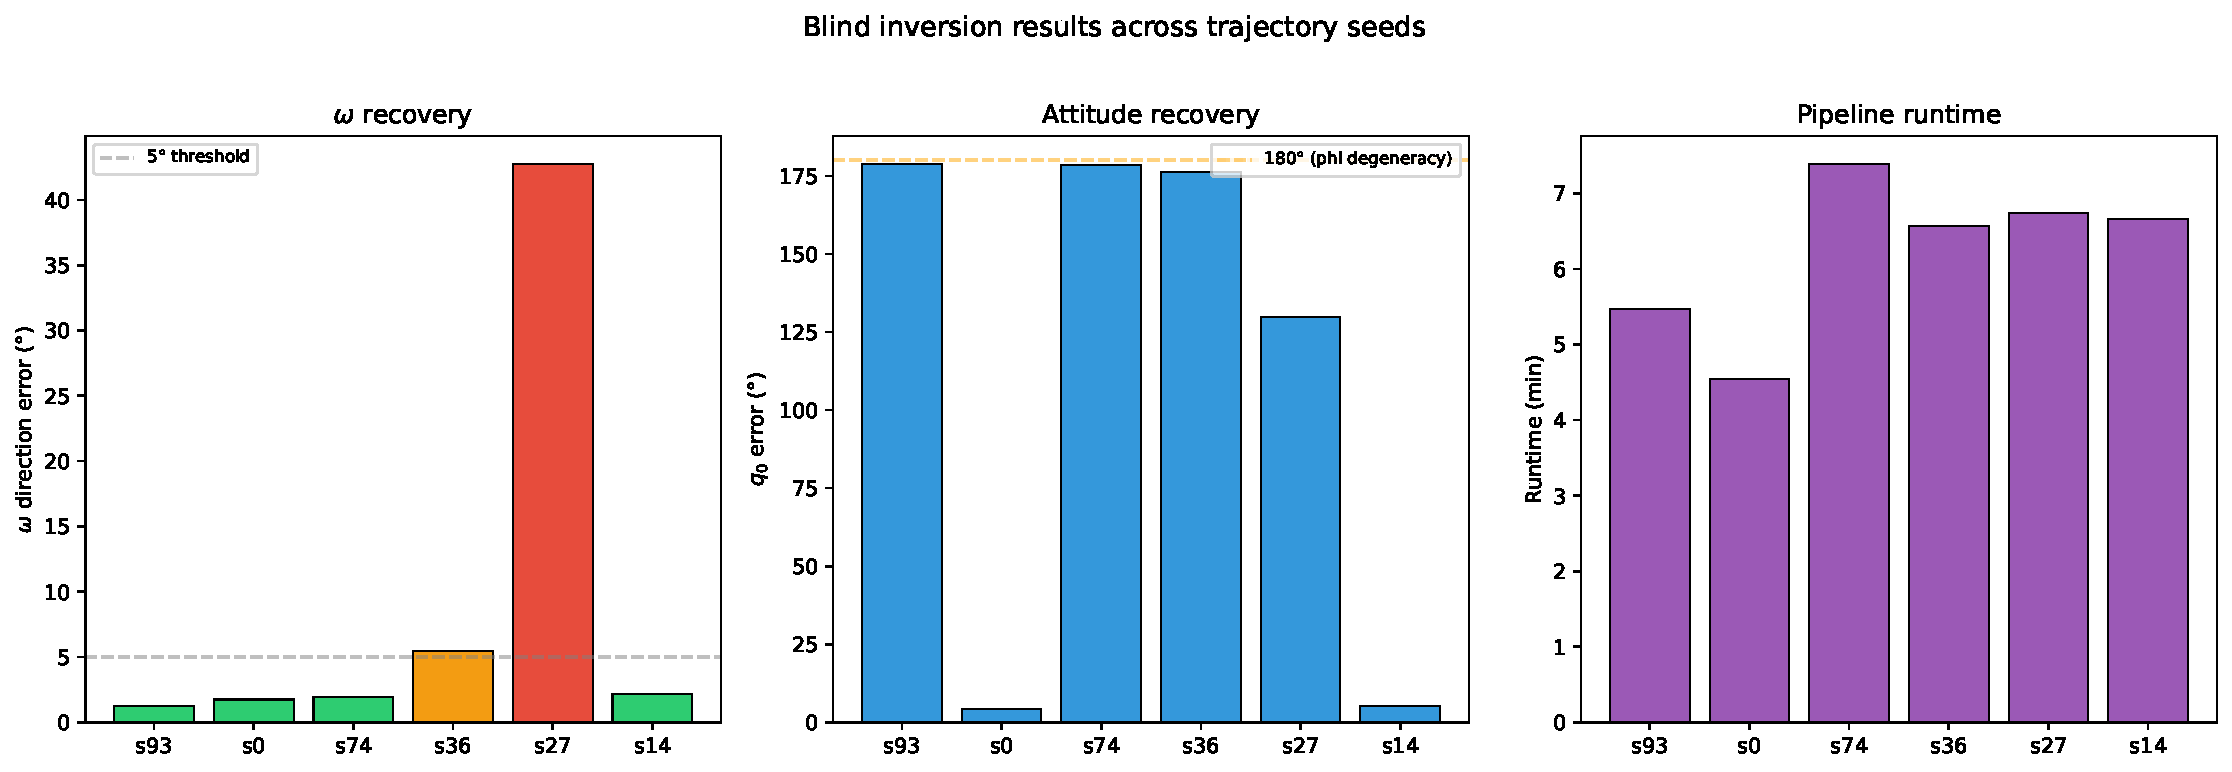
\includegraphics[width=\textwidth]{multiseed_summary.pdf}
\caption{$\omega$ direction error, attitude error, and runtime across seeds.
Green: $< 5^\circ$. Orange: $5$--$20^\circ$. Red: $> 20^\circ$.}
\label{fig:multiseed}
\end{figure}

% ============================================================
\section{Next Steps}

\begin{itemize}[nosep]
  \item Restrict $\phi \in [0^\circ, 180^\circ)$ to eliminate the N/S
    degeneracy (halves candidate count)
  \item Larger seed sample ($\geq 20$ trajectories)
  \item Investigate failure mode for $n_\text{con} < 10$: denser grid or
    additional constraint types?
  \item Tune hand-picked parameters across the multi-seed set:
    alignment weights ($w_s = 10$, $w_b = 5$),
    NM candidate count (top 5 is arbitrary),
    grid density (2000 dirs, 20 mags --- magnitude axis is cheap to densify;
    ${\sim}0.5\%$ spacing (${\sim}80$ bins) costs little extra since
    propagation time is dominated by direction, not magnitude rescaling)
  \item Sensitivity to noise level and observation window length
\end{itemize}

\end{document}
